\noindent

\includegraphics[height=1.25cm]{images/pictograms/benchmark}

\includegraphics[height=1.25cm]{images/pictograms/tools}

\includegraphics[height=1.25cm]{images/pictograms/FEM}

\includegraphics[height=1.25cm]{images/pictograms/paraview}


%%%%%%%%%%%%%%%%%%%%%%%%%%%%%%%%%%%%%%%%%%%%%%%%%%%%%%%%%%%%%%%%%%%%%%%%%%%%%%%%%%%%%%%%%%%%%%%%%%%

\begin{flushright} {\tiny {\color{gray} python\_codes/fieldstone\_250/text.tex}} \end{flushright}

\lstinputlisting[language=bash,basicstyle=\small]{python_codes/fieldstone_150/keywords.key}

\par\noindent\rule{\textwidth}{0.4pt}

\begin{center}
\inpython
{\small Code: \url{https://github.com/cedrict/fieldstone/tree/master/python_codes/fieldstone_150}}
\end{center}

\par\noindent\rule{\textwidth}{0.4pt}

%%%%%%%%%%%%%%%%%%%%%%%%%%%%%%%%%%%%%%%%%%%%%%%%%%%%%%%%%%%%%%%%%%%%%%%%%%%%%%%%%%%%%%%%%%%%%%%%%%%

This \stone is an attempt at looking into the optimisation of how (FE) stones have been coded 
up until now. In particular I want to try to build the (Stokes) FE matrix much faster.
If successful, this would enable either higher resolution runs, or longer time series, 
or a quicker way to steady state, etc ...

We then start from the {\pythonfile stone\_V0.py} script which solves the 
Donea \& Huerta benchmark (see \ref{mmm:mms1}) in a unit square by means of \QtwoQone elements.
It is very similar to \stone~\ref{f48} for example.

%%%%%%%%%%%%%%%%%%%%%%%%%%%%%%%%%%%%%%%%%%%%%%%%%
\section*{Standard approach}

Running the model at resolution $128 \times 128$ elements, we find that building 
the matrix takes approximately 11.7s and solving the system approximatively 1.4s.  
Although the solve time grows like $nel^{1.66}$, even running a $256\times 256$ elements model 
would still yields a build time that is substantially larger than the solve time.
Also, the part of the code which computes the $L_2$ errors can take up to a 
few seconds (in general 10x less time than building the matrix).
This is reason enough to try to make building the matrix {\it much} faster.
Although there is no hard rule, it is commonly accepted that the solve is the 
most expensive part of a Stokes FE code.

\begin{center}
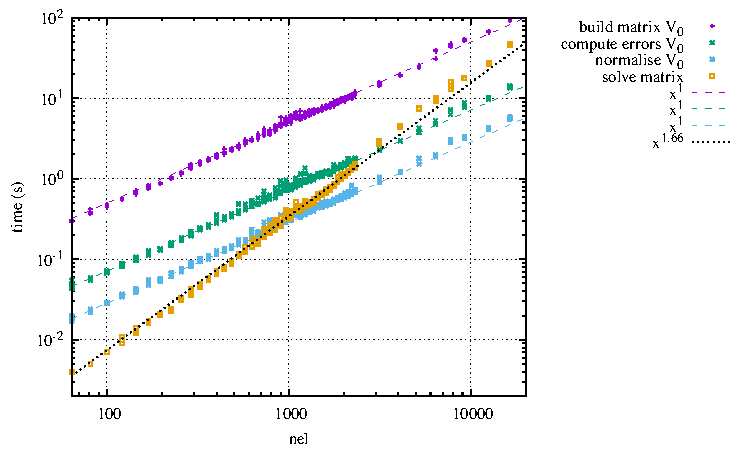
\includegraphics[width=8.5cm]{python_codes/fieldstone_150/results/times_V0}
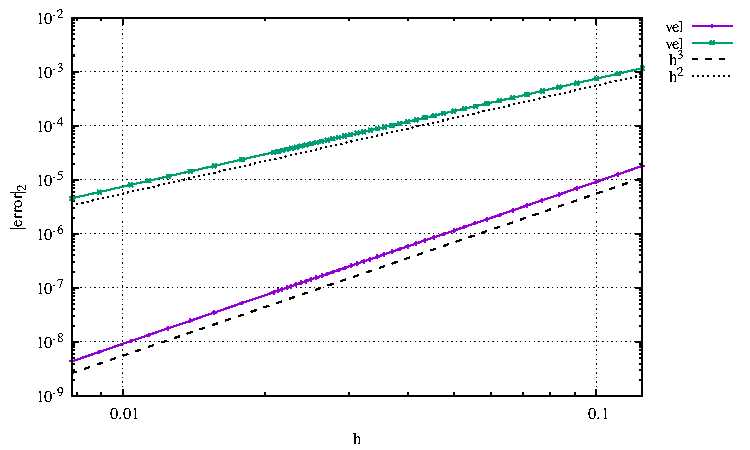
\includegraphics[width=8.5cm]{python_codes/fieldstone_150/results/errors_V0}\\
{\captionfont 
Left: Timings of 4 parts of the code as a function of the number of elements.
Right: $L_2$-error convergence plot as a function of the element size $h$.
}
\end{center}



%%%%%%%%%%%%%%%%%%%%%%%%%%%%%%%%%%%%%%%%%%%%%%%%%
\section*{Dealing with the Jacobian matrix code bits}

To start with I here assume that we are dealing with rectangular elements, 
all of the same size $(h_x,h_y)$. This allows to replace this typical piece of code 
\begin{lstlisting}
for iel in range(0,nel):
    for iq in range(0,nqperdim):
        for jq in range(0,nqperdim):
            ...
            jcb=np.zeros((ndim,ndim),dtype=np.float64)
            for k in range(0,mV):
                jcb[0,0] += dNNNVdr[k]*xV[iconV[k,iel]]
                jcb[0,1] += dNNNVdr[k]*yV[iconV[k,iel]]
                jcb[1,0] += dNNNVds[k]*xV[iconV[k,iel]]
                jcb[1,1] += dNNNVds[k]*yV[iconV[k,iel]]
            jcob = np.linalg.det(jcb)
            jcbi = np.linalg.inv(jcb)
\end{lstlisting}
by something much simpler. Indeed, in this case the Jacobian matrix is 
\[
{\bm J}=\left(
\begin{array}{cc}
h_x/2 & 0 \\ 0 & h_y/2
\end{array}
\right)
\]
so that the determinant is $|{\bm J}|=h_xh_y/4$ and its inverse:
\[
{\bm J}^{-1}
=\left(
\begin{array}{cc}
2/h_x & 0 \\ 0 & 2/h_y
\end{array}
\right)
\]
We can then replace the code excerpt above (which is usually called at every quadrature 
of every element) by:
\begin{lstlisting}
jcbi=np.zeros((ndim,ndim),dtype=np.float64)
jcbi[0,0]=2/hx
jcbi[1,1]=2/hy
jcob=hx*hy/4

for iel in range(0,nel):
    for iq in range(0,nqperdim):
        for jq in range(0,nqperdim):
            ...

\end{lstlisting}
Note that the explicit calculation of the Jacobian determinant and inverse
is also present in the pressure normalisation and error calculations.

This is very simple and 
is carried out in {\pythonfile stone\_V1.py}.

\begin{center}
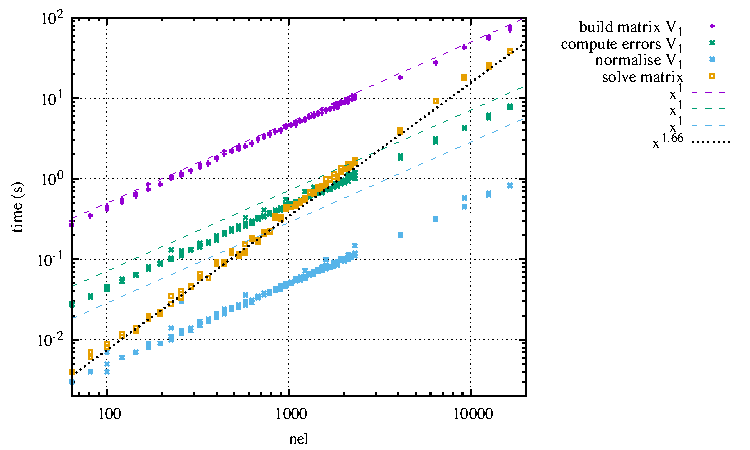
\includegraphics[width=8.5cm]{python_codes/fieldstone_150/results/times_V1}\\
{\captionfont Timings of 4 parts of the code as a function of the number of elements.
The dotted lines correspond to the timings of version V0.}
\end{center}

\begin{center}
\begin{tabular}{lcc}
\hline
& V0 & V1 \\
\hline
\hline
build matrix      ($128\times 128$)& 77.3-82.4 s&  69.7-78 s \\
normalise pressure($128\times 128$)&           s&  0.81-0.84 s\\
compute errors    ($128\times 128$)& 12.2-12.9 s& 7.6-8 s    \\
\hline
\end{tabular}
\end{center}

We see that this change has not really lead to a substantial improvement in 
computational time, especially for the build time (only 10\% improvement)... 

%%%%%%%%%%%%%%%%%%%%%%%%%%%%%%%%%%%%%%%%%%%%%%%%%
\section*{Dealing with the basis functions}

In about every FE code so far, we encounter this bit:

\begin{lstlisting}
NNNV    = np.zeros(mV,dtype=np.float64) 
NNNP    = np.zeros(mP,dtype=np.float64) 
dNNNVdr = np.zeros(mV,dtype=np.float64) 
dNNNVds = np.zeros(mV,dtype=np.float64) 

for iel in range(0,nel):
    for iq in range(0,nqperdim):
        for jq in range(0,nqperdim):
            rq=qcoords[iq]
            sq=qcoords[jq]
            weightq=qweights[iq]*qweights[jq]

            NNNV[0:mV]=NNV(rq,sq)
            dNNNVdr[0:mV]=dNNVdr(rq,sq)
            dNNNVds[0:mV]=dNNVds(rq,sq)
            NNNP[0:mP]=NNP(rq,sq)
\end{lstlisting}
If we look at it more closely, we see that the basis functions are evaluated for every 
element at the (here) 9 reduced coordinates of the quadrature points. 
We should then instead precompute the values of the basis functions at the 
reduced coordinates of the {\tt nqel}={\tt nqperdim**ndim} quadrature points as follows:

\begin{lstlisting}
NNNV    = np.zeros((nqel,mV),dtype=np.float64) 
NNNP    = np.zeros((nqel,mP),dtype=np.float64) 
dNNNVdr = np.zeros((nqel,mV),dtype=np.float64) 
dNNNVds = np.zeros((nqel,mV),dtype=np.float64) 
rq = np.zeros(nqel,dtype=np.float64) 
sq = np.zeros(nqel,dtype=np.float64) 
weightq = np.zeros(nqel,dtype=np.float64) 
   
counterq=0 
for iq in range(0,nqperdim):
    for jq in range(0,nqperdim):
        rq[counterq]=qcoords[iq]
        sq[counterq]=qcoords[jq]
        weightq[counterq]=qweights[iq]*qweights[jq]
        NNNV[counterq,0:mV]=NNV(rq,sq)
        dNNNVdr[counterq,0:mV]=dNNVdr(rq,sq)
        dNNNVds[counterq,0:mV]=dNNVds(rq,sq)
        NNNP[counterq,0:mP]=NNP(rq,sq)
        counterq+=1
\end{lstlisting}
so that we can later reuse these where needed (note that we have transformed the 
double for loop on quadrature points into a single one):
\begin{lstlisting}
for iel in range(0,nel):
    for iq in range(0,nqel):
        ...
        rq[iq],sq[iq],weightq[iq]
        NNNV[iq,0:mV]
        dNNNVdr[iq,0:mV]
        dNNNVds[iq,0:mV]
        NNNP[iq,0:mP]
\end{lstlisting}

Looking further down we then see that the inverse of the Jacobian matrix 
is used to compute the derivatives of the basis functions in the real 
coordinate space $(x,y)$:
\begin{lstlisting}
for k in range(0,mV):
    dNNNVdx[k]=jcbi[0,0]*dNNNVdr[k]+jcbi[0,1]*dNNNVds[k]
    dNNNVdy[k]=jcbi[1,0]*dNNNVdr[k]+jcbi[1,1]*dNNNVds[k]
\end{lstlisting}
From what follows above we know that {\tt jcbi[0,1]} and {\tt jcbi[1,0]} are 
both zero, so that in fact we have 
\begin{lstlisting}
for k in range(0,mV):
    dNNNVdx[k]=jcbi[0,0]*dNNNVdr[k]
    dNNNVdy[k]=jcbi[1,1]*dNNNVds[k]
\end{lstlisting}
which means that these too can be precomputed at the quadrature points before entering 
the loop over elements:
\begin{lstlisting}
NNNV    = np.zeros((nqel,mV),dtype=np.float64) 
NNNP    = np.zeros((nqel,mP),dtype=np.float64) 
dNNNVdr = np.zeros((nqel,mV),dtype=np.float64) 
dNNNVds = np.zeros((nqel,mV),dtype=np.float64) 
dNNNVdx = np.zeros((nqel,mV),dtype=np.float64) 
dNNNVdy = np.zeros((nqel,mV),dtype=np.float64) 
rq = np.zeros(nqel,dtype=np.float64) 
sq = np.zeros(nqel,dtype=np.float64) 
weightq = np.zeros(nqel,dtype=np.float64) 
 
counterq=0 
for iq in range(0,nqperdim):
    for jq in range(0,nqperdim):
        rq[counterq]=qcoords[iq]
        sq[counterq]=qcoords[jq]
        weightq[counterq]=qweights[iq]*qweights[jq]
        NNNV[counterq,0:mV]=NNV(rq,sq)
        dNNNVdr[counterq,0:mV]=dNNVdr(rq,sq)
        dNNNVds[counterq,0:mV]=dNNVds(rq,sq)
        NNNP[counterq,0:mP]=NNP(rq,sq)
        dNNNVdx[counterq,0:mV]=jcbi[0,0]*dNNNVdr[counterq,0:mV]
        dNNNVdy[counterq,0:mV]=jcbi[1,1]*dNNNVds[counterq,0:mV]
        counterq+=1

for iel in range(0,nel):
    for iq in range(0,nqel):
        ...
\end{lstlisting}
All of this now happens only once, before entering the element loop!
This means that inside the element loop and the quadrature point loop, 
only the calculation of $\K_e$, the boundary conditions and the assembly 
must take place.
In the very specific case that the viscosity is constant (at least within each element)
one could also precompute $\K_e/\eta_e$ beforehand for example. 
Another interesting option would be to compute $\K_e$ for a linear viscosity in the
element given by $\eta_e(x,y)=a+bx+cy$ (think symbolic calculation ?).

This is carried out in {\pythonfile stone\_V2.py}.


\begin{center}
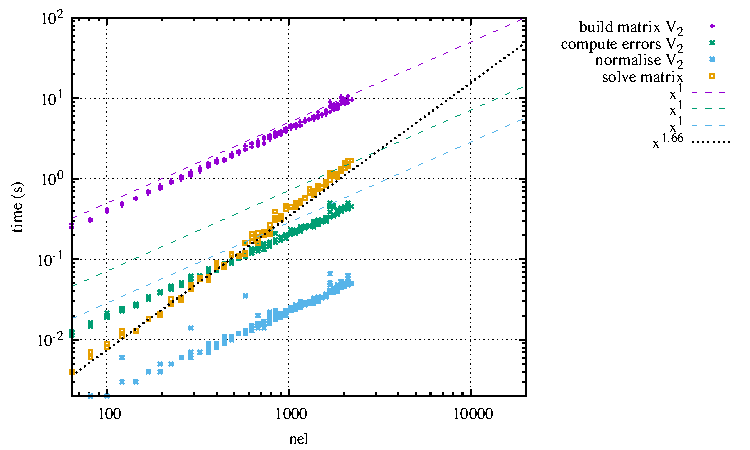
\includegraphics[width=8.5cm]{python_codes/fieldstone_150/results/times_V2}\\
{\captionfont Timings of 4 parts of the code as a function of the number of elements.
The dotted lines correspond to the timings of version V0.}
\end{center}

Here two, we see that we have improved the timings of the normalisation and 
error calculations but not of the matrix building. 
One possible benefit from this is that the code is getting more compact.
Note that of course we can verify that the measured errors themselves have not changed.
 
Side note: in the calculation of errors (and elsewhere), we had so far these explicit loops:

\begin{lstlisting}
for iel in range (0,nel):
    for iq in range(0,nqel):
        xq=0.
        yq=0.
        uq=0.
        vq=0.
        qq=0.
        for k in range(0,mV):
            xq+=
            yq+=NNNV[iq,k]*yV[iconV[k,iel]]
            uq+=NNNV[iq,k]*u[iconV[k,iel]]
            vq+=NNNV[iq,k]*v[iconV[k,iel]]
            qq+=NNNV[iq,k]*q[iconV[k,iel]]
        errv+=((uq-velocity_x(xq,yq))**2+(vq-velocity_y(xq,yq))**2)*weightq[iq]*jcob
        errq+=(qq-pressure(xq,yq))**2*weightq[iq]*jcob
\end{lstlisting}
This is easily replaced by a much more compact code:
\begin{lstlisting}
for iel in range (0,nel):
    for iq in range(0,nqel):
        xq=np.dot(NNNV[iq,:],xV[iconV[:,iel]])
        yq=np.dot(NNNV[iq,:],yV[iconV[:,iel]])
        uq=np.dot(NNNV[iq,:],u[iconV[:,iel]])
        vq=np.dot(NNNV[iq,:],v[iconV[:,iel]])
        qq=np.dot(NNNV[iq,:],q[iconV[:,iel]])
        errv+=((uq-velocity_x(xq,yq))**2+(vq-velocity_y(xq,yq))**2)*weightq[iq]*jcob
        errq+=(qq-pressure(xq,yq))**2*weightq[iq]*jcob
\end{lstlisting}
Such approach has been taken where ever possible in the stone.
This makes bits of code even more compact (we have lost 30+ lines so far).
As it turns out, this is also much faster (about 30\%), as shown here for
the error calculations:
\begin{center}
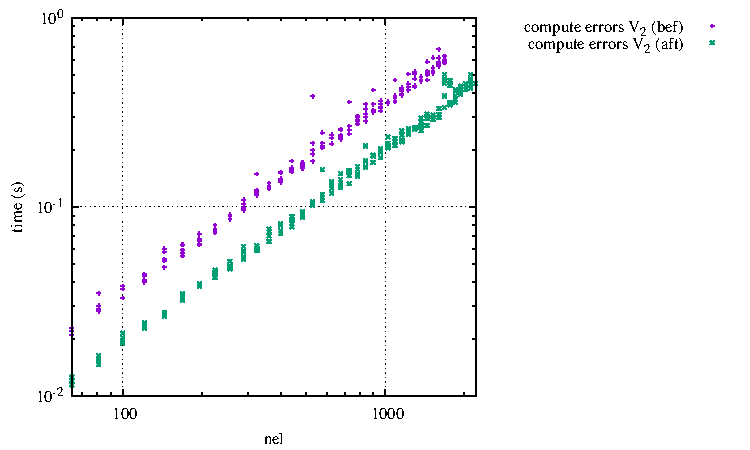
\includegraphics[width=8.5cm]{python_codes/fieldstone_150/results/times_V2_errors}
\end{center}

All in all, there is an improvement in the timings, but nothing really 
substantial with regards to the matrix building. Let's dig deeper. 


%%%%%%%%%%%%%%%%%%%%%%%%%%%%%%%%%%%%%%%%%%%%%%%%%
\section*{Improving matrix building (1)}

We see that in the V2 version we have 
\begin{lstlisting}
for i in range(0,mP):
    N_mat[0,i]=NNNP[iq,i]
    N_mat[1,i]=NNNP[iq,i]
    N_mat[2,i]=0.
\end{lstlisting}
which can be replaced by
\begin{lstlisting}
N_mat[0,0:mP]=NNNP[iq,0:mP]
N_mat[1,0:mP]=NNNP[iq,0:mP]
\end{lstlisting}
but it barely registers in terms on compute time. 
As this stage we have the building matrix code that looks as 
follows:
\begin{lstlisting}
for iel in range(0,nel):
    loop over qpts to build K_el,G_el,f_el
    impose boundary conditions
    assemble
\end{lstlisting}
The question is then: which part is the most costly?
In order to have an idea, we can implement something like this:
\begin{lstlisting}
for iel in range(0,nel):
    start1 = timing.time()
    loop over qpts to build K_el,G_el,f_el
    end1 = timing.time()
    --
    start2 = timing.time()
    impose boundary conditions
    end2 = timing.time()
    --
    start3 = timing.time()
    assemble
    end3 = timing.time()
    --
    t1+=end1-start1
    t2+=end2-start2
    t3+=end3-start3
\end{lstlisting}
This is carried out in {\pythonfile stone\_V3.py}.
This is probably not ideal since these calls probably slow the execution 
of the element loop somewhat, but it proves to be informative:
\begin{center}
\begin{tabular}{lccccc}
\hline
resolution & t1 & t2 & t3 & t1+t2+t3 & t3/t1\\ 
\hline
\hline
$32\times 32$   & 0.90  s& 0.06 s& 3.12  s& 4.08  s & 3.3\\ 
$48\times 48$   & 1.93  s& 0.11 s& 6.61  s& 9.24  s & 3.4\\
$96\times 96$   & 7.86  s& 0.40 s& 26.34 s& 35.64 s & 3.4\\
$128\times 128$ & 13.87 s& 0.68 s& 47.04 s& 66.38 s & 3.5\\
\hline
\end{tabular}
\end{center}
The assembly seems to be the part that takes the most time (about 3x the quadrature points loop) so 
this is now our focus.

The assembly for each element looks like:
\begin{lstlisting}
for k1 in range(0,mV):
    for i1 in range(0,ndofV):
        ikk=ndofV*k1          +i1
        m1 =ndofV*iconV[k1,iel]+i1
        for k2 in range(0,mV):
            for i2 in range(0,ndofV):
                jkk=ndofV*k2          +i2
                m2 =ndofV*iconV[k2,iel]+i2
                A_sparse[m1,m2] += K_el[ikk,jkk]
\end{lstlisting}
Effectively the loops over {\tt k1+i1} and {\tt k2+i2} loop over all terms of the {\tt K\_el}.
Since we know that explicit for loops are slow in python, we could try to rewrite this as follows:
\begin{lstlisting}
for ikk in range(0,ndofV*mV): 
    for jkk in range(0,ndofV*mV): 
        A_sparse[X,Y] += K_el[ikk,jkk]
\end{lstlisting}
where the values X and Y have been precomputed for each element. 
In the case of \QtwoQone elements in 2D, we have mV=9 and ndofV=2 so that 
the size of the matrix {\tt K\_el} is $18\times 18$. For each of these 18 dofs 
I need to know its corresponding global dof number. 
I can precompute this for each element as follows:
 
\begin{lstlisting}
local_to_globalV=np.zeros((ndofV_el,nel),dtype=np.int32)
for iel in range(0,nel):
    for k1 in range(0,mV):
        for i1 in range(0,ndofV):
            ikk=ndofV*k1          +i1
            m1 =ndofV*iconV[k1,iel]+i1
            local_to_globalV[ikk,iel]=m1
\end{lstlisting}
and the assembly has now become more compact:
\begin{lstlisting}
    for ikk in range(ndofV_el):
        m1=local_to_globalV[ikk,iel]
        for jkk in range(ndofV_el):
            A_sparse[m1,local_to_globalV[jkk,iel]] += K_el[ikk,jkk]
        for jkk in range(0,mP):
            m2 =iconP[jkk,iel]
            A_sparse[m1,NfemV+m2]+=G_el[ikk,jkk]
            A_sparse[NfemV+m2,m1]+=G_el[ikk,jkk]
        f_rhs[m1]+=f_el[ikk]
    for k2 in range(0,mP):
        m2=iconP[k2,iel]
        h_rhs[m2]+=h_el[k2]
\end{lstlisting}
This is carried out in {\pythonfile stone\_V4.py}. Unfortunately, 
the improvement is just not very substantial again (a few percents at best).

\begin{center}
\begin{tabular}{lccccc}
\hline
resolution & t1 & t2 & t3 & t1+t2+t3 & t3/t1\\ 
\hline
\hline
$32\times 32$   &  0.88 s& 0.05 s&  2.11 s&  3.04 s& 2.40 \\ 
$48\times 48$   &  2.04 s& 0.11 s&  4.96 s&  7.12 s& 2.42 \\
$96\times 96$   &  7.90 s& 0.40 s& 18.80 s& 27.11 s& 2.38 \\
$128\times 128$ & 14.32 s& 0.72 s& 35.93 s& 50.97 s& 2.51 \\
\hline
\end{tabular}
\end{center}

Turning now to the calculation of the elemental matrices, 
I put a timer around each piece of code:
\begin{lstlisting}
    for iq in range(0,nqel):

        start11 = timing.time()
        xq=np.dot(NNNV[iq,:],xV[iconV[:,iel]])
        yq=np.dot(NNNV[iq,:],yV[iconV[:,iel]])
        end11 = timing.time()

        start12 = timing.time()
        for i in range(0,mV):
            b_mat[0:3, 2*i:2*i+2] = [[dNNNVdx[iq,i],0.           ],
                                     [0.           ,dNNNVdy[iq,i]],
                                     [dNNNVdy[iq,i],dNNNVdx[iq,i]]]
        end12 = timing.time()

        start13 = timing.time()
        K_el+=b_mat.T.dot(c_mat.dot(b_mat))*eta*weightq[iq]*jcob
        end13 = timing.time()

        start14 = timing.time()
        for i in range(0,mV):
            f_el[ndofV*i  ]+=NNNV[iq,i]*jcob*weightq[iq]*bx(xq,yq)
            f_el[ndofV*i+1]+=NNNV[iq,i]*jcob*weightq[iq]*by(xq,yq)
        end14 = timing.time()

        start15 = timing.time()
        N_mat[0,0:mP]=NNNP[iq,0:mP]
        N_mat[1,0:mP]=NNNP[iq,0:mP]
        end15 = timing.time()

        start16 = timing.time()
        G_el-=b_mat.T.dot(N_mat)*weightq[iq]*jcob
        end16 = timing.time()

        t11+=end11-start11
        t12+=end12-start12
        t13+=end13-start13
        t14+=end14-start14
        t15+=end15-start15
        t16+=end16-start16

    # end for iq
\end{lstlisting}
I found that t14 was rather large, but it actually comes from 
the complicated polynomial calculations inside bx and by. 
The second most costly was t12. A lucky guess had me replace
\begin{lstlisting}
for i in range(0,mV):
    b_mat[0:3, 2*i:2*i+2] = [[dNNNVdx[iq,i],0.           ],
                             [0.           ,dNNNVdy[iq,i]],
                             [dNNNVdy[iq,i],dNNNVdx[iq,i]]]
\end{lstlisting}
by 
\begin{lstlisting}
for i in range(0,mV):
    b_mat[0,2*i  ]=dNNNVdx[iq,i]
    b_mat[1,2*i+1]=dNNNVdy[iq,i]
    b_mat[2,2*i  ]=dNNNVdy[iq,i]
    b_mat[2,2*i+1]=dNNNVdx[iq,i]
\end{lstlisting}
and I obtained an improvement for t1:
\begin{center}
\begin{tabular}{lccccc}
\hline
resolution & t1 & t2 & t3 & t1+t2+t3 & t3/t1\\ 
\hline
\hline
$32\times 32$   &  0.77 & 0.05 &  2.06 &  2.89 & 2.69 \\
$48\times 48$   &  1.75 & 0.11 &  4.92 &  6.79 & 2.81 \\
$96\times 96$   &  7.26 & 0.42 & 19.97 & 27.65 & 2.75 \\
$128\times 128$ &  12.66& 0.67 & 35.13 & 48.46 & 2.77 \\ 
\hline
\end{tabular}
\end{center}
Again, nothing spectacular.
Looking at this block again, we see that we have 4 times the occurence of the product {\tt jcob*weightq[iq]}.
We should therefore compute it once and store it:
\begin{lstlisting}
JxW=jcob*weightq[iq]
\end{lstlisting}

All in all, this is where we are at:
\begin{center}
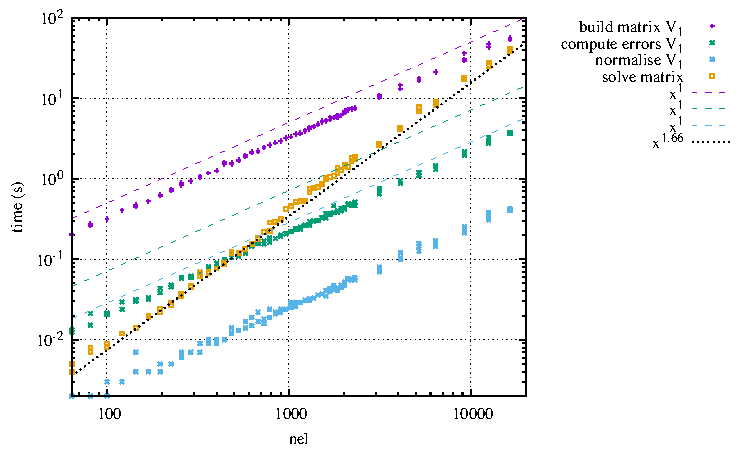
\includegraphics[width=8.5cm]{python_codes/fieldstone_150/results/times_V4}
\end{center}
The matrix build for 128x128 used to take about 80s for V0, now it takes 
about 55s. Let us be honest, I was hoping for at least a factor 2. 

%%%%%%%%%%%%%%%%%%%%%%%%%%%%%%%%%%%%%%%%%%%%%%%%%
\section*{Dealing with the matrix storage}

One thing we have not tried yet is to not use a linked list approach to store the 
FE matrix but instead use a full array approach, i.e.
 
\begin{lstlisting}
A_sparse=np.zeros((Nfem,Nfem),dtype=np.float64)
...
sparse_matrix=sps.csr_matrix(A_sparse)
\end{lstlisting}
instead of 
\begin{lstlisting}
A_sparse=lil_matrix((Nfem,Nfem),dtype=np.float64)
...
sparse_matrix=A_sparse.tocsr()
\end{lstlisting}
This is carried out in {\pythonfile stone\_V5.py}. 
\begin{center}
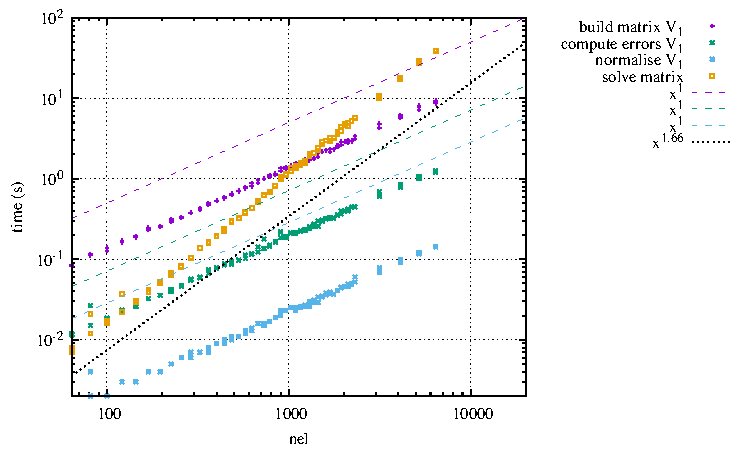
\includegraphics[width=8.5cm]{python_codes/fieldstone_150/results/times_V5}
\end{center}
The build time is improved BUT there are two problems: a) converting the matrix to csr 
format before passing it to the solver takes more time and therefore shifts the solve
time up; b) the simulation stops at resolution 96x96 as the python interpreter complains 
about the memory to store the matrix:
``Unable to allocate 165. GiB for an array with shape (148739, 148739) and data type float64''.

%%%%%%%%%%%%%%%%%%%%%%%%%%%%%%%%%%%%%%%%%%%%%%%%%
\section*{Not giving up on matrix assembly}

Upon searching online, I came across this example:

\begin{lstlisting}
from scipy import sparse
from numpy import array
I = array([0,0,1,3,1,0,0])
J = array([0,2,1,3,1,0,0])
V = array([1,1,1,1,1,1,1])
B = sparse.coo_matrix((V,(I,J)),shape=(4,4)).tocsr()
\end{lstlisting}
This is straightforward: keep a list of the integer coordinates of the nonzeros and their values
in a large array and let the class {\tt coo\_matrix} assemble it all in a large matrix.
This is also explained there\footnote{\url{https://stackoverflow.com/questions/10522296/how-to-assemble-large-sparse-matrices-effectively-in-python-scipy}}.

In our case the size of these arrays will be large.
They will contain {\it all} the values of all $\K_e$ and $\G_e$!
I have written a short script {\pythonfile compute\_sizes.py} which computes the required memory to store these arrays:

\begin{lstlisting}
nel=256**2
ndofV=2
mV=9
mP=4
size=nel*( (mV*ndofV)**2 + 2*(mV*ndofV*mP) )
print('array size=',size)
print('--> arrays I,J are int32')
print('    ',size*32,'bits')
print('    ',size*32/8,'bytes')
print('    ',size*32/8/1024,'kbytes')
print('    ',size*32/8/1024/1024,'Mbytes')
print('    ',size*32/8/1024/1024/1024,'Gbytes')

print('--> array V is float64')
print('    ',size*64,'bits')
print('    ',size*64/8,'bytes')
print('    ',size*64/8/1024,'kbytes')
print('    ',size*64/8/1024/1024,'Mbytes')
print('    ',size*64/8/1024/1024/1024,'Gbytes')
\end{lstlisting}
We then get for a 256x256 mesh of \QtwoQone elements:
\begin{verbatim}
array size= 30670848
--> arrays I,J are int32
     981467136 bits
     122683392.0 bytes
     119808.0 kbytes
     117.0 Mbytes
     0.1142578125 Gbytes each
--> array V is float64
     1962934272 bits
     245366784.0 bytes
     239616.0 kbytes
     234.0 Mbytes
     0.228515625 Gbytes
\end{verbatim}
or, less than a Gb of memory to store it all!


This is carried out in {\pythonfile stone\_V6.py}. 
and the assembly then looks like:
\begin{lstlisting}
bignb=nel*((mV*ndofV)**2+2*(mV*ndofV*mP))

I=np.zeros(bignb,dtype=np.int32)    
J=np.zeros(bignb,dtype=np.int32)    
V=np.zeros(bignb,dtype=np.float64)    

counter=0
for iel in range(0,nel):

    ... build K_el
    ... apply boundary conditions

    for ikk in range(ndofV_el):
        m1=local_to_globalV[ikk,iel]
        for jkk in range(ndofV_el):
            m2=local_to_globalV[jkk,iel]
            I[counter]=m1
            J[counter]=m2
            V[counter]=K_el[ikk,jkk]
            counter+=1
        for jkk in range(0,mP):
            m2 =iconP[jkk,iel]+NfemV
            I[counter]=m1
            J[counter]=m2
            V[counter]=G_el[ikk,jkk]
            counter+=1
            I[counter]=m2
            J[counter]=m1
            V[counter]=G_el[ikk,jkk]
            counter+=1
        f_rhs[m1]+=f_el[ikk]
    for k2 in range(0,mP):
        m2=iconP[k2,iel]
        h_rhs[m2]+=h_el[k2]
    end3 = timing.time()

sparse_matrix = sparse.coo_matrix((V,(I,J)),shape=(Nfem,Nfem)).tocsr()
\end{lstlisting}

Also, filling {\tt I} and {\tt J} can be done once and for all if the 
mesh topology does not change
which is always the case in our codes. This therefore takes place before the loop over 
elements which would represent a gain in the case of time stepping or nonlinear iterations
when the FE matrix needs to be rebuilt multiple times.

In the end, the assembly process is very compact:
\begin{lstlisting}
bignb=nel*((mV*ndofV)**2+2*(mV*ndofV*mP))

I=np.zeros(bignb,dtype=np.int32)    
J=np.zeros(bignb,dtype=np.int32)    
V=np.zeros(bignb,dtype=np.float64)    

...fill I,J

counter=0
for iel in range(0,nel):

    ... build K_el
    ... apply boundary conditions

    for ikk in range(ndofV_el):
        m1=local_to_globalV[ikk,iel]
        for jkk in range(ndofV_el):
            V[counter]=K_el[ikk,jkk]
            counter+=1
        for jkk in range(0,mP):
            V[counter]=G_el[ikk,jkk]
            counter+=1
            V[counter]=G_el[ikk,jkk]
            counter+=1
        f_rhs[m1]+=f_el[ikk]
    for k2 in range(0,mP):
        m2=iconP[k2,iel]
        h_rhs[m2]+=h_el[k2]
    end3 = timing.time()

sparse_matrix = sparse.coo_matrix((V,(I,J)),shape=(Nfem,Nfem)).tocsr()
\end{lstlisting}

Note that the last line has been incorporated in the solve timing 
since it replaces the previous command which 
transformed the lil matrix into csr format.

\begin{center}
\begin{tabular}{lccccc}
\hline
resolution & t1 & t2 & t3 & t1+t2+t3 & t3/t1\\ 
\hline
\hline
$32\times 32$   &  0.70 & 0.05 & 0.14 &  0.90 & 0.21 \\
$48\times 48$   &  1.62 & 0.11 & 0.33 &  2.06 & 0.21 \\
$96\times 96$   &  6.33 & 0.38 & 1.28 &  8.00 & 0.20 \\
$128\times 128$ & 12.24 & 0.71 & 2.55 & 15.50 & 0.21 \\
\hline
\end{tabular}
\end{center}

Compared to V3, t3 has gone from 47s to less than 3s!
Results are finally substantial! the matrix build 
has nearly decreased by a factor of 5 with respect to V0
while the solve time remains indentical!
But now we need to look again at t1, i.e. the making of the 
element matrices $\K_e$ and $\G_e$. In the $128\times 128$ case the call to bx,by 
costs about 7s from the 12s of t1, so that in the case of a buoyancy 
driven flow with for example $g_x=0$ and $g_y=-g_0$ then t1 would be 
about 5s. 

\begin{center}
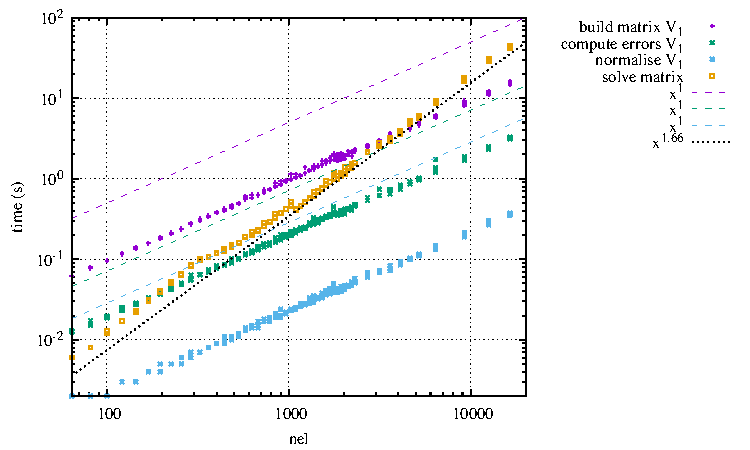
\includegraphics[width=8.5cm]{python_codes/fieldstone_150/results/times_V6}
\end{center}


%-------------------------------------------------------------------------
\section*{Back to computing elemental matrices / looking at b.c.}

I have tried replacing in {\pythonfile stone\_V7.py} 
\begin{lstlisting}
for i in range(0,mV):
    b_mat[0,2*i  ]=dNNNVdx[iq,i]
    b_mat[1,2*i+1]=dNNNVdy[iq,i]
    b_mat[2,2*i  ]=dNNNVdy[iq,i]
    b_mat[2,2*i+1]=dNNNVdx[iq,i]
\end{lstlisting}
by 
\begin{lstlisting}
for i in range(0,mV):
    dNdx=dNNNVdx[iq,i] 
    dNdy=dNNNVdy[iq,i] 
    b_mat[0,2*i  ]=dNdx
    b_mat[1,2*i+1]=dNdy
    b_mat[2,2*i  ]=dNdy
    b_mat[2,2*i+1]=dNdx
\end{lstlisting}
and found a minor improvement (few percents on t12).

I have then tried 
\begin{lstlisting}
b_mat[0,:]=[dNNNVdx[iq,0],0,dNNNVdx[iq,1],0,dNNNVdx[iq,2],0,\
            dNNNVdx[iq,3],0,dNNNVdx[iq,4],0,dNNNVdx[iq,5],0,\
            dNNNVdx[iq,6],0,dNNNVdx[iq,7],0,dNNNVdx[iq,8],0]
b_mat[1,:]=[0,dNNNVdy[iq,0],0,dNNNVdy[iq,1],0,dNNNVdy[iq,2],\
            0,dNNNVdy[iq,3],0,dNNNVdy[iq,4],0,dNNNVdy[iq,5],\
            0,dNNNVdy[iq,6],0,dNNNVdy[iq,7],0,dNNNVdy[iq,8]]
b_mat[2,:]=[dNNNVdy[iq,0],dNNNVdx[iq,0],\
            dNNNVdy[iq,1],dNNNVdx[iq,1],\
            dNNNVdy[iq,2],dNNNVdx[iq,2],\
            dNNNVdy[iq,3],dNNNVdx[iq,3],\
            dNNNVdy[iq,4],dNNNVdx[iq,4],\
            dNNNVdy[iq,5],dNNNVdx[iq,5],\
            dNNNVdy[iq,6],dNNNVdx[iq,6],\
            dNNNVdy[iq,7],dNNNVdx[iq,7],\
            dNNNVdy[iq,8],dNNNVdx[iq,8]]
\end{lstlisting}
which is of course ugly and not extendable to 3D or higher order elements. 
It did not yield any improvement at all so I abandoned this.

Likewise I replaced
\begin{lstlisting}
for i in range(0,mV):
    f_el[ndofV*i  ]+=NNNV[iq,i]*JxW*bx(xq,yq)
    f_el[ndofV*i+1]+=NNNV[iq,i]*JxW*by(xq,yq)
\end{lstlisting}
by 
\begin{lstlisting}
for i in range(0,mV):
    Ni=NNNV[iq,i]i*JxW
    f_el[ndofV*i  ]+=Ni*bx(xq,yq)
    f_el[ndofV*i+1]+=Ni*by(xq,yq)
\end{lstlisting}
and shave off a few percents off t14.

Finally, we can also make use of the {\tt local\_to\_globalV}
array in the boundary conditions, so that 
\begin{lstlisting}
for k1 in range(0,mV):
    for i1 in range(0,ndofV):
        ikk=ndofV*k1          +i1
        m1 =ndofV*iconV[k1,iel]+i1
        if bc_fix[m1]:
           ...
\end{lstlisting}
is replaced by
\begin{lstlisting}
for ikk in range(0,ndofV_el):
    m1=local_to_globalV[ikk,iel]
    if bc_fix[m1]:
       ...
\end{lstlisting}
Once again, this is more compact and contains less nested loops.

\begin{center}
\begin{tabular}{lccccc}
\hline
resolution & t1 & t2 & t3 & t1+t2+t3 & t3/t1\\ 
\hline
\hline
$32\times 32$   &   0.71 s& 0.019 s& 0.14 s&  0.87 s& 0.20 \\  
$48\times 48$   &   1.54 s& 0.034 s& 0.32 s&  1.90 s& 0.21 \\
$96\times 96$   &   6.23 s& 0.094 s& 1.38 s&  7.71 s& 0.22 \\
$128\times 128$ &  10.82 s& 0.140 s& 2.29 s& 13.25 s& 0.21 \\
\hline
\end{tabular}
\end{center}
We see that the boundary conditions time has been divided by 5!


\begin{center}
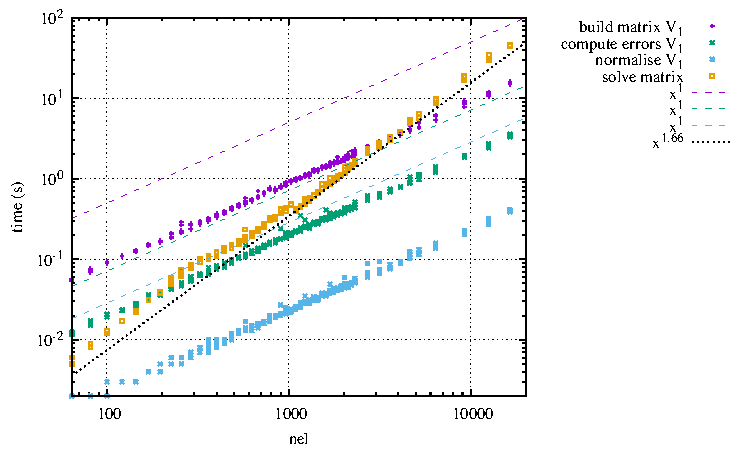
\includegraphics[width=8.5cm]{python_codes/fieldstone_150/results/times_V7}
\end{center}

\begin{center}
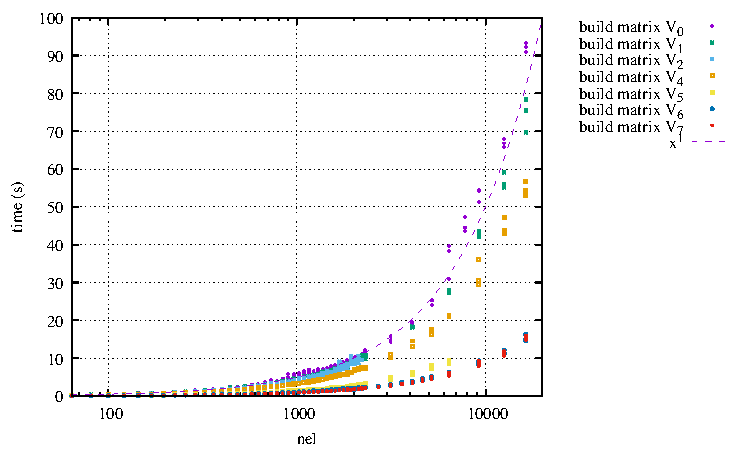
\includegraphics[width=8.5cm]{python_codes/fieldstone_150/results/times_build_all}
\end{center}



%%%%%%%%%%%%%%%%%%%%%%%%%%%%%%%%%%%%%%%%%%%%%%%%%%%%%%%%%%%%%%%%%%%%%%%%%%%%%%%%%%%%%%%%%%%%%%%%%%%
\par\noindent\rule{\textwidth}{0.4pt}

\vspace{.5cm}

\begin{center}
\fbox{\begin{minipage}{0.9\textwidth}
{\color{teal}To Do, open questions, future work?}
\begin{itemize}
\item do smthg
\end{itemize}
\end{minipage}}
\end{center}

%%%%%%%%%%%%%%%%%%%%%%%%%%%%%%%%%%%%%%%%%%%%%%%%%%%%%%%%%%%%%%%%%%%%%%%%%%%%%%%%%%%%%%%%%%%%%%%%%%%
\vspace{.5cm}

Note that there is quite some literature about how to carry out the assembly in a very efficient 
manner. 
\begin{itemize}
\item \fullcite{cujs16}
\item \fullcite{voet23}
\end{itemize}


